%%
%  ******************************************************************************
%  * #file    Szablon_raportu_EN_Latex.tex
%  * #author  Adrian Wójcik   adrian.wojcik(at)put.poznan.pl
%  *          
%  * #commit  Patryk Kościk   koscikpatryk(at)gmail.com
%  *          Modified the template for Projekt przejsciowy purposes          
%  *          
%  * #version 1.0
%  * #date    09-Mar-2022
%  * #brief   PROJPRZEJ
%  *
%  ******************************************************************************
%%  
\documentclass[11pt, a4paper]{article}

\usepackage{SM_template}

% Wypełnijcie te dyrektywy zgodnie z waszym tematem
% \lab      -> NAZWA CZUJNIKA, np.: 'DHT22'
% \comment  -> Króciutki opis co to, np.: 'Cyfrowy budżetowy czujnik temperatury'
%
\lab{Moduł KY-006}
\comment{Buzzer pasywny}

% Absolutny zakaz dotykania tego tutaj bo jak dotkiecie to coś jebnie
\university{Politechnika Poznańska}
\faculty{Wydział Automatyki, Robotyki i Elektrotechniki}
\institute{Instytut Robotyki i Inteligencji Maszynowej}
\department{Zakład Sterowania i Elektroniki Przemysłowej}
\addbibresource{bib/Kontaktron-KY-006.bib}
\nocite{*}


%%
%
% Początek dokumentu
%
%%
\begin{document}

%% Strona tytułowa %%
\mainpage{{Kontaktron-KY-006/zdj_modułu/tytulowa.jpg}}
\newpage

\section{Opis elementu} \addcontentsline{toc}{section}{Wstęp}
Głównym elementem modułu KY-006 jest buzzer pasywny, inaczej nazywany też brzęczykiem. W przypadku omawianego modułu jest to buzzer wykorzystujący odwrotne zjawisko piezoelektryczne. Pod wpływem podawania zmieniającego się napięcia na materiał wewnątrz brzęczyka wpada on w drgania, co powoduje powstanie fali dźwiękowej. Buzzery pasywne w celu wytwarzania dźwięku wymagają zmieniającego się napięcia na wejściu sygnałowym, co odróżnia je od buzzerów aktywnych, które wystarczy włączyć stanem wysokim, aby wytwarzały dźwięk.
% \vspace{0.3cm}
% \begin{figure}[H]
% \centering
% 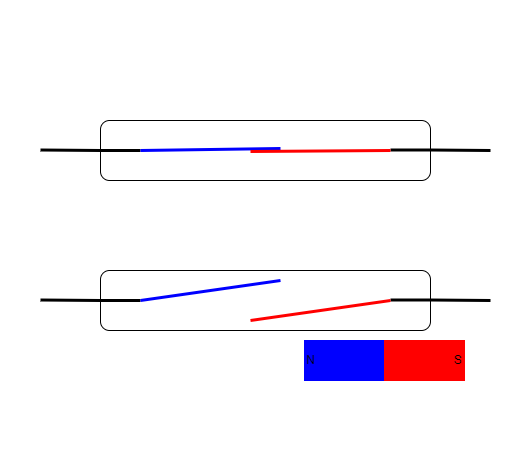
\includegraphics[width=.7\linewidth]{fig/Kontaktron-KY-006/zasada_dzialania/zasada_dzialania.png}
% \caption{}
% \label{fig:sub3}
% \end{figure}
% \vspace{0.3cm}

\begin{figure}[H]
\centering
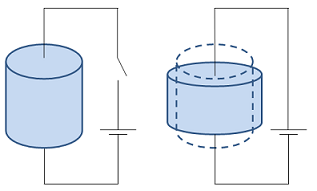
\includegraphics[width=.5\linewidth]{fig/Kontaktron-KY-006/zasada_dzialania/piezoelectric_inverse_effect.png}
\caption{Odwrotny efekt piezoelektryczny\cite{piezo_effect}}
\label{fig:sub3}
\end{figure}



\subsection{Opis modułu}
Moduł KY-006 zbudowany jest z 3 pinów (sygnałowy, napięcie zasilania, masa), z czego wykorzystywane są tylko 2 (pin zasilania nie jest wykorzystywany), oraz samego buzzera.
\begin{figure}[H]
\centering
\begin{subfigure}{.5\textwidth}
  \centering
  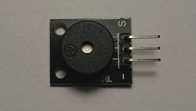
\includegraphics[width=.6\linewidth]{fig/Kontaktron-KY-006/zdj_modułu/widok_z_gory_bok.jpg}
  \label{fig:sub1}
  \caption{Zdjęcie modułu KY-006}
\end{subfigure}%
\begin{subfigure}{.5\textwidth}
  \centering
  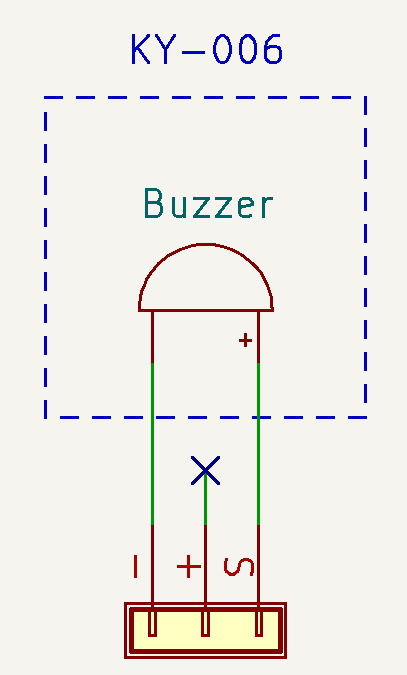
\includegraphics[width=.5\linewidth]{fig/Kontaktron-KY-006/zasada_dzialania/schemat_ukladu.PNG}
  \label{fig:sub2}
  \caption{Schemat elektryczny modułu}
\end{subfigure}
%\caption{Połączenie elektryczne}
\label{fig:test}
\end{figure}

\subsection{Zastosowania}
Buzzer pasywny, dzięki możliwości zmieniania częstotliwości jego dźwięku, można wykorzystać do alarmowania o różnych błędach w układzie(inna częstotliwość w zależności od typu błędu). Poza tym aspektem buzzery pasywne można wykorzystać w ten sam sposób co aktywne, póki jest dostęp do sygnału PWM (lub innego o zmiennej wartości napięcia w czasie).



\newpage
\hypersetup{
    colorlinks=true,
    linkcolor=blue,
    filecolor=magenta,      
    urlcolor=cyan,
    pdftitle={Overleaf Example},
    pdfpagemode=FullScreen,
    }
\section{Użycie czujnika}
W celu zaprezentowania działania modułu posłużono się płytką Nucleo F746ZG, na której skonfigurowano kanał 1 licznika TIM3, tak aby generował sygnał PWM na pin PB4. 

\vspace{0.3cm}
\begin{figure}[H]
\centering
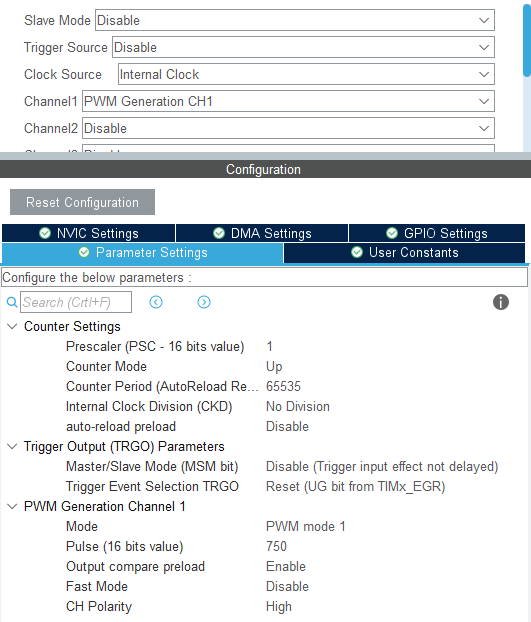
\includegraphics[width=.7\linewidth]{fig/Kontaktron-KY-006/działanie_ukladu/przykladoweIOC.PNG}
\caption{Przykładowa konfiguracja timera w CubeIDE}
\label{fig:sub3}
\end{figure}
\vspace{0.3cm}
\vspace{0.3cm}
\begin{figure}[H]
\centering
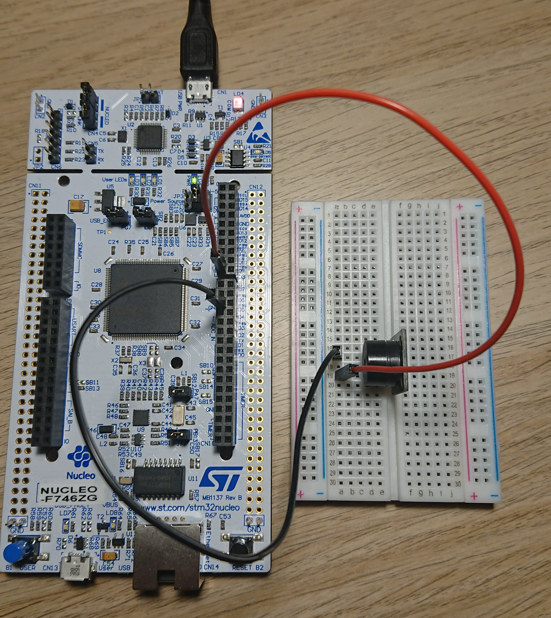
\includegraphics[width=.7\linewidth]{fig/Kontaktron-KY-006/działanie_ukladu/polaczenie.PNG}
\caption{Połączenie układu z płytką STM32. Czerwony kabel łączy pin licznika z wejściem sygnałowym buzzera}
\label{fig:sub3}
\end{figure}
\vspace{0.3cm}

\printbibliography[heading=bibintoc]

\end{document}